\chapter{Transfer function measurement software}\label{appendix:transfer_function}
In this appendix the transfer function measurement routine will be explained briefly. The goal of this software is to be able to compute the impulse response of a \gls{dut} using the logarithmic swept sine method and compute the transfer function from the impulse response. To be able to send out a logarithmic swept sine signal and measure an input signal at the same time, a full duplex soundcard has to be utilized as the measuring soundcard. In order to be able to reproduce every measurement and compare measurements, the chosen soundcard model will not be changed doing the project.

\section*{Materials and setup}
To measure the transfer function of a \gls{dut}, the following materials are used:
\begin{itemize}
\item RME FIREFACE ucx (Soundcard)
\begin{itemize}[noitemsep]
\item AAU-number: 108230
\item Serial number: 23811948
\end{itemize}
\item MATLAB 2017b (PC - software)
\item \gls{usb} A to \gls{usb} B cable
\end{itemize}



\begin{figure}[H]
\centering
\begin{picture}(0,0)%
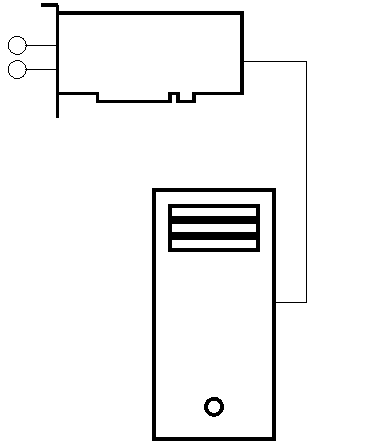
\includegraphics{transfer_function.pdf}%
\end{picture}%
\setlength{\unitlength}{2818sp}%
%
\begingroup\makeatletter\ifx\SetFigFont\undefined%
\gdef\SetFigFont#1#2#3#4#5{%
  \reset@font\fontsize{#1}{#2pt}%
  \fontfamily{#3}\fontseries{#4}\fontshape{#5}%
  \selectfont}%
\fi\endgroup%
\begin{picture}(4090,4926)(8176,-7474)
\put(8191,-3661){Out}%
\put(9271,-3211){Sound Card}%
\put(9971,-6361){Computer}%
\put(11836,-4696){USB}%
\put(8281,-2806){In}%
\end{picture}%
\caption{Setup for measuring transfer function}
		\label{fig:appendix:transfer_function}
\end{figure}

\section*{Transfer function software}
The software is made as a function where the impulse response and transfer function and a time and frequency x-axis vector are returned respectively. The function name is:

\includeCode{IRmeas_fft.m}{matlab}{1}{1}{The turntable control function}{code:IRmeas_fft_function}{./code/sine_swept/}

To get output from this function, the following variable have to be initialised.



 \begin{table}[H]
\centering
\caption{Function command}
\label{my-label}
\begin{tabular}{lll}
 & \texttt{ts} & Length of the logarithmic swept sine in {[}\SI{}{\second}{]} \\
 & \texttt{ttw} & Duration that is recorded after the end of the sweep in {[}\SI{}{\second}{]}    \\
 & \texttt{tflower} & Lower frequency border for logarithmic swept sine in {[}\SI{}{\hertz}{]}  \\
 & \texttt{tfupper} & Upper frequency border for logarithmic swept sine in {[}\SI{}{\hertz}{]} \\
 & \texttt{tplaygain} & Gain relativ to digital \texttt{1} for sweep playback in {[}\SI{}{\decibel}{]} \\
 & \texttt{tplayer}  & I-O system object for playback and record via the soundcard
\end{tabular}
\end{table}



\section*{The MATLAB function}
\includeCode{IRmeas_fft.m}{matlab}{1}{82}{The turntable control function}{code:IRmeas_fft}{./code/sine_swept/}

